\documentclass[10pt]{article}
\usepackage[margin=0.62in]{geometry}
\usepackage{amsmath,amssymb,booktabs,graphicx}
\usepackage[hidelinks]{hyperref}
\setlength{\parindent}{0pt}
\setlength{\parskip}{3pt}
\setlength{\abovedisplayskip}{4pt}
\setlength{\belowdisplayskip}{4pt}
\setlength{\textfloatsep}{7pt}
\setlength{\floatsep}{6pt}
\renewcommand{\arraystretch}{1.08}

\title{\vspace{-1.3cm}\textbf{Controlling $2+2\!\to\!4$ Circuit Formation\\
with a Parent-Only First Block}}
\author{}
\date{\vspace{-1.15cm}}

\begin{document}
\maketitle
\vspace{-0.75cm}

\textbf{Summary.}
We derive a zero-temperature stationary phase diagram for a two-block residual ReLU network
with independent weight decays, under the explicit restriction that block 1 produces the two
supervised $d2$ parents but no $d4$ feature.  At fixed representation strengths $(s,q)$, we
analytically eliminate the parent readouts, the block-2 target-producing weights, and the $d4$
readout.  We then minimize the resulting scalar free energy over $(s,q)$ separately for the
direct $1+1+1+1\to4$ and compositional $2+2\to4$ circuits.  The familiar condition
$Q_2/Q_1^{(1)}>1/\sqrt8$ selects composition only at a fixed representation; the phase of the
trainable model is instead determined by comparing the two complete minima of $\Phi+G$.

\section*{1. Model and assumptions}
For target parity $\chi_a(x)\in\{-1,+1\}$, let $f_a(x)=w_a^\top h_2(x)$ and define its
target-mode amplitude $\widehat A_a=\mathbb E_x[f_a(x)\chi_a(x)]$.  Under the pure aligned-mode
ansatz $f_a=\widehat A_a\chi_a$, the sample loss reduces as
$\mathbb E_x[(f_a-\chi_a)^2]=(1-\widehat A_a)^2$, since $\chi_a^2=1$.  The network and
reduced weighted objective are therefore
\begin{align}
h_1&=h_0+\sigma(V_1h_0),& h_2&=h_1+\sigma(V_2h_1),\nonumber\\[-2pt]
f_a&=w_a^\top h_2,\nonumber\\[-5pt]
\mathcal J&=\frac{\gamma_2}{2}\!\sum_{a\in\{12,34\}}(1-\widehat A_a)^2
+\frac{\gamma_4}{2}(1-\widehat A_4)^2
+\frac12\!\left(\lambda_E\|E\|^2+\lambda_1\|V_1\|^2+\lambda_2\|V_2\|^2\right.\nonumber\\[-2pt]
&\hspace{4.2cm}\left.+\lambda_p\|W_{d2}\|^2+\lambda_4\|w_4\|^2\right).
\label{eq:objective}
\end{align}
The derivation assumes: (A1) the full four-bit cube and pure ReLU; (A2) four equal-norm,
orthogonal singleton Walsh vectors of norm $s=Q_1^{(0)}$; (A3) two equal-norm, orthogonal
parent vectors $q_{12},q_{34}$ of norm $q=Q_2$; (A4) balanced rank-one gates, sufficient
width, and additive parameter norms for parent and target sectors; (A5) the block-2 target
vector aligns with its $d4$ readout; (A6) block 1 is restricted to the parent sector and
produces no $d4$ feature; and (A7) the global zero-temperature minimum is reached.  Thus this is an equilibrium
mode theory, not a claim about finite-time SGD or dynamical lock-in.

The symbol $V_1$ in Eq.~\eqref{eq:objective} is the \emph{entire} first-block weight matrix.
Under assumptions A4 and A6, we decompose it conceptually as
\begin{equation}
V_1=V_{1,\rm parent}+V_{1,\rm other},\qquad
\|V_1\|_F^2=\|V_{1,\rm parent}\|_F^2+\|V_{1,\rm other}\|_F^2.
\label{eq:v1-decomp}
\end{equation}
$V_{1,\rm parent}$ is not a separate network parameter.  It denotes the minimum-norm component
of $V_1$ that implements the two supervised $1+1\to2$ parent gates.  Assumption A6 removes the
block-1 $d4$ sector rather than assigning it a finite cost; this is the simplifying restriction
that avoids lower-mode leakage from a block-1 four-input ReLU.

The singleton byproduct of an ideal parent gate is not a fitted parameter:
\begin{equation}
\sigma\!\left[a(x_1+x_2)\right]
=\frac a2(1+x_1+x_2+x_1x_2).
\label{eq:relu-decomp}
\end{equation}
It has the same singleton and pair coefficient.  If this generated singleton vector is
orthogonal to the residual singleton vector, then
\begin{equation}
Q_1^{(1)}=\sqrt{s^2+q^2}.
\label{eq:q1out}
\end{equation}
For overlap $\rho$, replace $s^2+q^2$ by $s^2+q^2+2\rho sq$.  All gate-selection statements
below remain exact when expressed using the measured $Q_1^{(1)}$.

\section*{2. Derivation roadmap: what is minimized, and in what order}
The calculation is an algebraic elimination of weights from one simultaneous objective, not a
claim that training executes the following steps in time.  For each candidate block-2 target
circuit $r\in\{D,C\}$, the minimization is organized as follows.
\begin{enumerate}
\item Choose nonnegative order parameters $(s,q)$, where $s$ fixes the four singleton-feature
norms and $q$ fixes the two $d2$ parent-feature norms.
\item Holding $(s,q)$ fixed, minimize the $d2$ losses and the penalties on $E$,
$V_{1,\rm parent}$, and $W_{d2}$.  This gives the parent-sector free energy $\Phi(s,q)$.
\item Still holding $(s,q)$ fixed, choose either the direct block-2 circuit $D$ or the
compositional block-2 circuit $C$.  Minimize its hidden $d4$ norm and readout norm.  This gives
the target-sector free energy $G(\kappa_r)$.
\item Finally minimize $\Phi(s,q)+G(\kappa_r)$ over $(s,q)$.  The two families perform this
outer minimization separately, so their optimal representations need not be the same.  The
stationary phase is the family with lower final minimum.
\end{enumerate}
Schematically, the nested calculation is
\begin{equation}
F_r=\min_{s,q\geq0}\left[
\underbrace{\min_{B,\,E,V_{1,\rm parent},W_{d2}}\mathcal J_{d2}}_{\Phi(s,q)}+
\underbrace{\min_{Q\geq0,\,w_4}\mathcal J_{d4}}_{G(\kappa_r)}
\right],
\label{eq:roadmap}
\end{equation}
where $B$ is the common fitted amplitude of the two parent targets and
$Q=Q_{d4}^{(2)}$ is the norm of the $d4$ coefficient vector produced by block 2.

\section*{3. Eliminating weights: the two stationary free energies}
Equation~\eqref{eq:objective} specifies the penalties but does not by itself imply the norms
below; they are the minimum-norm realizations under A1--A4.  Write $e_i$ for the four
orthogonal singleton vectors.  Then $\|E\|_F^2=\sum_i\|e_i\|^2=4s^2$.  For one balanced
$1+1\to2$ gate of hidden norm $u$, the preactivation amplitude per parent is $us/\sqrt2$;
Eq.~\eqref{eq:relu-decomp} therefore gives $q=us/(2\sqrt2)$, or
$u^2=8q^2/s^2$.  The two disjoint parent gates add in squared norm.  Finally, the
minimum-norm readout satisfying $w_{ij}^{\top}q_{ij}=B$ is
$w_{ij}=Bq_{ij}/q^2$, with $\|w_{ij}\|^2=B^2/q^2$.  Thus the two readout rows also add, giving
\begin{equation}
\|E\|^2=4s^2,\qquad
\|V_{1,\rm parent}\|^2=\frac{16q^2}{s^2},\qquad
\|W_{d2}\|^2=\frac{2B^2}{q^2}.
\end{equation}
At fixed $(s,q)$, the parent-sector objective is therefore
\begin{equation}
\Phi(s,q)\equiv\min_{B\geq0}\left\{
\gamma_2(1-B)^2+2\lambda_Es^2+8\lambda_1\frac{q^2}{s^2}
+\lambda_p\frac{B^2}{q^2}\right\}.
\label{eq:phi-definition}
\end{equation}
This definition includes both $d2$ losses and the regularization needed to create and read out
the singleton and parent representations.  It excludes every $d4$-specific weight and the
$d4$ loss.  Minimizing the displayed expression over the common parent amplitude gives
\begin{align}
B^*(q)&=\frac{\gamma_2q^2}{\gamma_2q^2+\lambda_p},\nonumber\\[-2pt]
\Phi(s,q)&=2\lambda_Es^2+8\lambda_1\frac{q^2}{s^2}
+\frac{\gamma_2\lambda_p}{\gamma_2q^2+\lambda_p}.
\label{eq:parent-free}
\end{align}

The two allowed target circuits are now both in block 2: $D$ is the direct
$1+1+1+1\to4$ circuit and $C$ is the compositional $2+2\to4$ circuit.  Their efficiencies
per target-producing hidden-weight norm $u_r$ are
\begin{equation}
Q=\eta_r u_r,\qquad
\eta_D=\frac{Q_1^{(1)}}{8}=\frac{\sqrt{s^2+q^2}}{8},\qquad
\eta_C=\frac{Q_2^{(1)}}{2\sqrt2}=\frac{q}{2\sqrt2}.
\label{eq:etas}
\end{equation}
Because the hidden penalty is $\lambda_2u_r^2/2$, producing a hidden $d4$ norm $Q$ costs
$\kappa_rQ^2/2$, where the cost per squared target-mode norm is
\begin{equation}
\kappa_r\equiv\frac{\lambda_2}{\eta_r^2},\qquad
\kappa_D=\frac{64\lambda_2}{s^2+q^2},\qquad
\kappa_C=\frac{8\lambda_2}{q^2}.
\label{eq:kappas}
\end{equation}
Thus smaller $\kappa_r$ means a more efficient circuit.

Let $t=\|w_4\|$.  Under the aligned pure-mode ansatz, the fitted target amplitude is $tQ$,
so at fixed $(s,q)$ the target objective is
\begin{equation}
\mathcal J_{4,r}(Q,t)=\frac{\gamma_4}{2}(1-tQ)^2
+\frac{\lambda_4}{2}t^2+\frac{\kappa_r}{2}Q^2.
\label{eq:target-objective}
\end{equation}
Minimizing first over the readout norm gives
\begin{equation}
t^*(Q)=\frac{\gamma_4Q}{\gamma_4Q^2+\lambda_4},\qquad
\min_t\mathcal J_{4,r}(Q,t)=\frac{\kappa_r}{2}Q^2
+\frac{\gamma_4\lambda_4}{2(\gamma_4Q^2+\lambda_4)}.
\label{eq:readout-eliminated}
\end{equation}
The remaining minimization over $Q\geq0$ yields
\begin{equation}
(Q_r^*)^2=\left[\sqrt{\frac{\lambda_4}{\kappa_r}}
-\frac{\lambda_4}{\gamma_4}\right]_+.
\label{eq:q4-optimum}
\end{equation}
The target is active precisely when
\begin{equation}
\kappa_r\lambda_4<\gamma_4^2;\qquad
\kappa_r\lambda_4\geq\gamma_4^2\ \Longrightarrow\ Q_r^*=0.
\label{eq:activity}
\end{equation}
Substitution gives the target-sector free energy directly in terms of the circuit cost:
\begin{equation}
G(\kappa_r)=
\begin{cases}
\sqrt{\kappa_r\lambda_4}-\dfrac{\kappa_r\lambda_4}{2\gamma_4},
&\kappa_r\lambda_4<\gamma_4^2,\\[6pt]
\dfrac{\gamma_4}{2},&\kappa_r\lambda_4\geq\gamma_4^2.
\end{cases}
\label{eq:target-free}
\end{equation}
The corresponding fitted target amplitude is
\begin{equation}
A_r^*=t_r^*Q_r^*=\left[1-\frac{\sqrt{\kappa_r\lambda_4}}{\gamma_4}\right]_+.
\label{eq:target-amplitude}
\end{equation}
The closed phase theory is therefore
\begin{equation}
\boxed{F_D=\min_{s,q\geq0}\{\Phi(s,q)+G(\kappa_D(s,q))\},\qquad
F_C=\min_{s,q\geq0}\{\Phi(s,q)+G(\kappa_C(s,q))\}.}
\label{eq:free-energies}
\end{equation}
Each phase chooses its own representation; the joint-training transition $F_C=F_D$ can
therefore be first order even though the fixed-representation crossover is simple.

\section*{4. Phase diagram and control laws}
At fixed $(s,q)$, $G$ is nondecreasing in $\kappa$, so the cheaper block-2 circuit is selected by
\begin{equation}
\kappa_C<\kappa_D
\quad\Longleftrightarrow\quad
\frac{q}{\sqrt{s^2+q^2}}=\frac{Q_2}{Q_1^{(1)}}>\frac1{\sqrt8}.
\label{eq:boundary}
\end{equation}
This is only a conditional, fixed-representation crossover.  In the trainable model, the two
circuits generally choose different minimizers $(s_D,q_D)$ and $(s_C,q_C)$.  The actual phase
boundary is therefore
\begin{equation}
\boxed{F_C=F_D,}
\label{eq:global-boundary}
\end{equation}
with $F_D,F_C$ from Eq.~\eqref{eq:free-energies}.  The ratio test in
Eq.~\eqref{eq:boundary} becomes the full boundary only when $(s,q)$ is frozen, or when
$\Phi$ pins nearly the same representation for both circuits.  For a learned compositional
phase one must have
\begin{equation}
\boxed{F_C<F_D,\qquad \kappa_C(s_C,q_C)\lambda_4<\gamma_4^2.}
\label{eq:composition-conditions}
\end{equation}
The first condition compares the complete objectives after re-optimizing the representation;
the second prevents decay from suppressing the $d4$ target.  Equation~\eqref{eq:boundary}
must also hold at a strict compositional optimum, but by itself it is not sufficient.

\begin{figure}[h!]
\centering
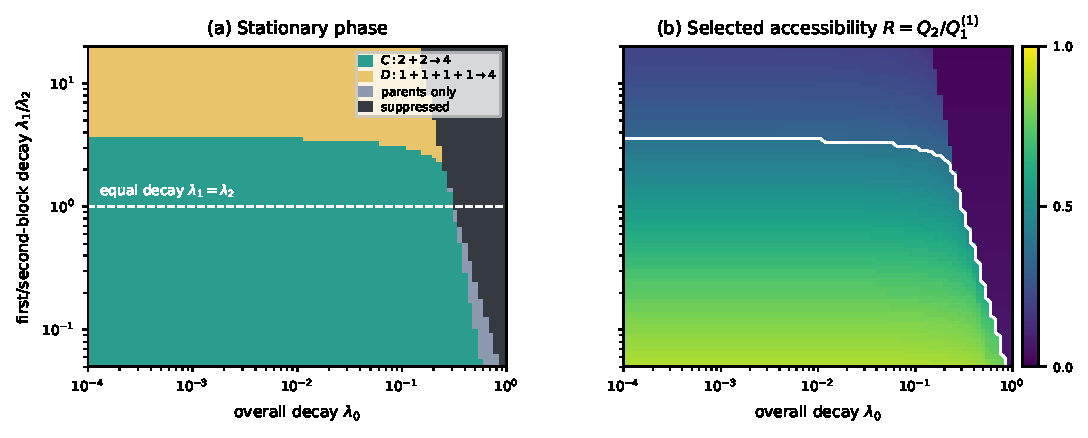
\includegraphics[width=0.99\textwidth]{fig_two_block_parent_only_layerwise_phase.pdf}
\vspace{-7pt}
\caption{\textbf{Canonical stationary phase diagram.}  We set
$\gamma_2=\gamma_4=2$, $\lambda_E=\lambda_p=\lambda_4=\lambda_2=\lambda_0$,
$\lambda_1/\lambda_2$ as the vertical control, and use assumptions A1--A7.
(a) Global minima of Eq.~\eqref{eq:free-energies}.  Excessive first-block decay destroys the
parents and favors the direct circuit; sufficiently large overall decay suppresses one or both
tasks.  (b) Accessibility $R=Q_2/Q_1^{(1)}$ at the selected global minimum.  The white contour
marks the fixed-representation crossover $R=1/\sqrt8$; the global phase boundary need not
coincide with it because the two families re-optimize $(s,q)$ separately.}
\label{fig:phase}
\end{figure}

\textbf{How to tune the restricted trainable model.}
(1) Decay $w_4$; without it, hidden/readout rescaling invalidates norm comparison.
(2) Preserve the parents with strong $d2$ supervision and modest $\lambda_E,\lambda_1,
\lambda_p$ until the \emph{final} measured $Q_2/Q_1^{(1)}$ exceeds $1/\sqrt8$.
(3) Avoid increasing $\lambda_1$ so far that the self-consistent parent norm $q$ collapses;
in this restricted model there is no block-1 $d4$ shortcut that benefits from large $\lambda_1$.
(4) Tune $\lambda_2\lambda_4$ below the activity threshold while retaining nonzero decay on
both factors.  This controls target formation but does not alter the local $1/\sqrt8$ crossover.
(5) Compare the complete measured objective of the direct and compositional solutions; the
final accessibility ratio alone is not a global phase test when all parent weights remain trainable.

\begin{center}
\begin{tabular}{@{}lll@{}}
\toprule
Control & Desired movement & Limiting failure \\
\midrule
$\lambda_1\!\downarrow$ & preserve or enlarge $d2$ parents & large block-1 norms \\
$\lambda_2\!\downarrow$ & lower both block-2 circuit costs & large block-2 norms \\
$\lambda_p\!\downarrow$ or $\gamma_2\!\uparrow$ & preserve $d2$ parents & weak parent regularization \\
$\lambda_4\!\downarrow$ & keep the $d4$ target active & large readout norm \\
$\lambda_E\!\downarrow$ & preserve singleton sources & embedding norms grow \\
$\gamma_4\!\uparrow$ & relax the activity threshold & does not alone select $C$ \\
\bottomrule
\end{tabular}
\end{center}

\textbf{Scope.}
Nonzero singleton overlap $\rho$, unequal parent norms, imperfect target alignment, or
multifunctional neurons enlarge the order-parameter set.  Allowing block 1 to produce $d4$
invalidates assumption A6 and introduces an additional competing route and its lower-mode
byproducts.  Moreover, literal raw-ReLU parent and target gates emit constant and lower-degree
modes; the pure-mode ansatz assumes that unwanted output modes are projected out or cancelled,
and does not include the cost of that cancellation.  Finite-temperature Langevin
dynamics replaces $F_C=F_D$ by
$F_C-F_D+\tfrac{T}{2}\log(\det' H_C/\det' H_D)-T\log(g_C/g_D)=0$ and rounds the transition.
Ordinary full-batch SGD is effectively zero-noise but need not reach the global saddle, so
metastability and training history must be checked experimentally.

\end{document}
